\subsection{Triple Integrals}

\[
    \iiint_D f(x,y,z)\dd{V}
\]

Hard to visualize. If $f(x,y,z) = 1$:
\[
    \text{Volume of } D = \iiint_D 1\dd{V}
\]

Extend from 2D via Riemann sums --- think of density:
\[
    \iiint_{\text{Rect}} f
    = \lim_{\substack{l,m,n\to\infty}}
    \sum_{i=1}^{l}\sum_{j=1}^{m}\sum_{k=1}^{n}
    f(x_{ijk},\,y_{ijk},\,z_{ijk})\,\Delta x\,\Delta y\,\Delta z
\]
where $\Delta V = \Delta x\,\Delta y\,\Delta z$.

\begin{theorem}{Fubini's Theorem in 3D}{fubini-3d}
For a rectangular box $B = [a,b]\times[c,d]\times[r,s]$:
\[
    \iiint_B f(x,y,z)\dd{V}
    = \int_r^s\int_c^d\int_a^b f(x,y,z)\dd{x}\dd{y}\dd{z}
\]
\end{theorem}

\subsubsection{Type I Regions}

\begin{definition}{Type I Region}{type-i}
\[
    E = \{(x,y,z) \mid (x,y)\in D,\; u_1(x,y)\leq z\leq u_2(x,y)\}
\]
\end{definition}

\begin{center}
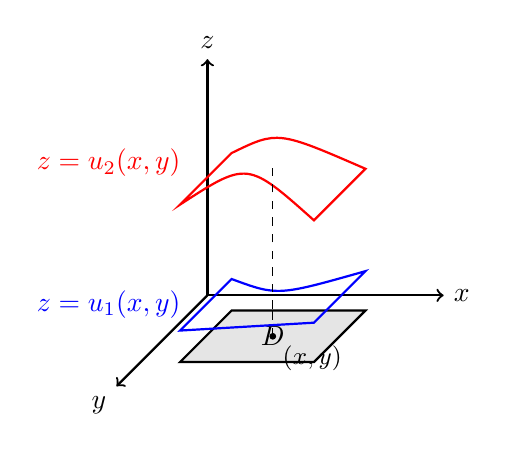
\begin{tikzpicture}
    \draw[thick,->] (0,0,0) -- (3,0,0) node[right]{$x$};
    \draw[thick,->] (0,0,0) -- (0,3,0) node[above]{$z$};
    \draw[thick,->] (0,0,0) -- (0,0,3) node[below left]{$y$};
    % projection D
    \draw[thick,fill=gray!20] (0.5,0,0.5) -- (2.2,0,0.5) -- (2.2,0,2.2) -- (0.5,0,2.2) -- cycle;
    \node at (1.35,0,1.35) {$D$};
    % lower surface
    \draw[thick,blue] (0.5,0.4,0.5) .. controls (1.2,0.3,0.8) .. (2.2,0.5,0.5)
        -- (2.2,0.5,2.2) .. controls (1.2,0.3,1.8) .. (0.5,0.4,2.2) -- cycle;
    \node[blue,left] at (0.3,0.4,1.35) {$z=u_1(x,y)$};
    % upper surface
    \draw[thick,red] (0.5,2.0,0.5) .. controls (1.2,2.4,0.8) .. (2.2,1.8,0.5)
        -- (2.2,1.8,2.2) .. controls (1.2,2.4,1.8) .. (0.5,2.0,2.2) -- cycle;
    \node[red,left] at (0.3,2.2,1.35) {$z=u_2(x,y)$};
    % vertical dashed line at sample point
    \draw[dashed] (1.35,0,1.35) -- (1.35,0.35,1.35);
    \draw[dashed] (1.35,0.35,1.35) -- (1.35,2.2,1.35);
    \filldraw (1.35,0,1.35) circle (1pt) node[below right]{\small$(x,y)$};
\end{tikzpicture}
\end{center}

Reduces 3D integral to 2D + 1D:
\[
    \iiint_E f\dd{V}
    = \iint_D\!\left(\int_{u_1(x,y)}^{u_2(x,y)} f\dd{z}\right)dA
\]

\begin{example}
$\displaystyle\iiint_E z\dd{V}$ where $E$ is the solid in $x,y,z\geq 0$ bounded by the surface $z = 12xy$ and the planes $y = x$, $x = 1$.

\begin{center}
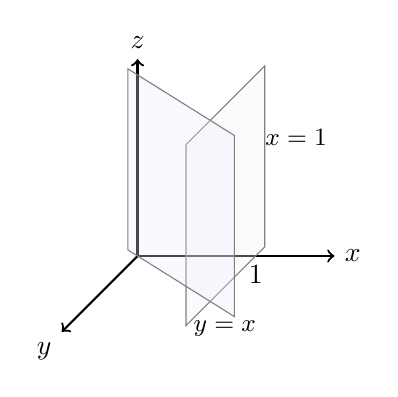
\begin{tikzpicture}
    % 3D sketch
    \draw[thick,->] (0,0,0) -- (2.5,0,0) node[right]{$x$};
    \draw[thick,->] (0,0,0) -- (0,2.5,0) node[above]{$z$};
    \draw[thick,->] (0,0,0) -- (0,0,2.5) node[below left]{$y$};
    % plane x=1 (vertical plane)
    \draw[gray,fill=gray!10,fill opacity=0.3]
        (1.5,0,-0.3) -- (1.5,0,2.3) -- (1.5,2.3,2.3) -- (1.5,2.3,-0.3) -- cycle;
    \node[below] at (1.5,0,0) {$1$};
    \node[right] at (1.5,1.5,0) {\small$x=1$};
    % plane y=x (vertical plane)
    \draw[gray,fill=blue!8,fill opacity=0.3]
        (-0.2,0,-0.2) -- (2.0,0,2.0) -- (2.0,2.3,2.0) -- (-0.2,2.3,-0.2) -- cycle;
    \node[below] at (1.8,0,1.8) {\small$y=x$};
\end{tikzpicture}
\hspace{1.5cm}
% D projection
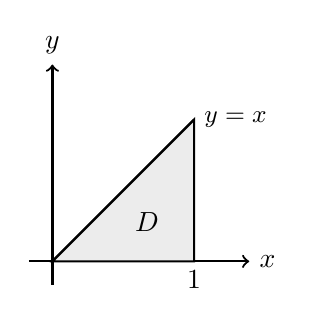
\begin{tikzpicture}
    \draw[thick,->] (-0.3,0) -- (2.5,0) node[right]{$x$};
    \draw[thick,->] (0,-0.3) -- (0,2.5) node[above]{$y$};
    \draw[thick] (0,0) -- (1.8,1.8) node[right]{\small$y=x$};
    \draw[thick] (1.8,0) -- (1.8,1.8);
    \draw[thick,fill=gray!15] (0,0) -- (1.8,1.8) -- (1.8,0) -- cycle;
    \node at (1.2,0.5) {$D$};
    \node[below] at (1.8,0) {$1$};
    \node[right] at (1.8,1.8) {};
\end{tikzpicture}
\end{center}

$D\colon\; 0\leq x\leq 1,\; 0\leq y\leq x$, \quad $z\colon\; 0\leq z\leq 12xy$.
\begin{align*}
    \iiint_E z\dd{V}
    &= \iint_D\!\left(\int_0^{12xy} z\dd{z}\right)dA
    = \int_0^1\!\int_0^x\!\int_0^{12xy} z\dd{z}\dd{y}\dd{x} \\
    &= \int_0^1\!\int_0^x \frac{z^2}{2}\bigg|_0^{12xy}\dd{y}\dd{x}
    = \int_0^1\!\int_0^x 72x^2y^2\dd{y}\dd{x} \\
    &= \int_0^1 72x^2\cdot\frac{y^3}{3}\bigg|_0^x\dd{x}
    = \int_0^1 24x^5\dd{x} \\
    &= 4x^6\big|_0^1
    = 4
\end{align*}
\end{example}

\begin{example}
Find the volume of the tetrahedron $T$ bounded by the planes $x + 2y + z = 2$, $x = 2y$, $x = 0$, $z = 0$.

\[
    \operatorname{Vol}(T) = \iiint_T 1\dd{V}
\]

\begin{center}
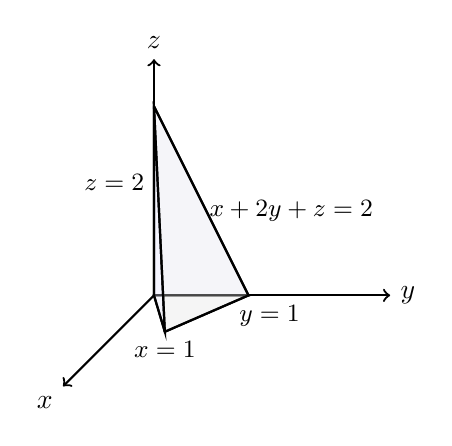
\begin{tikzpicture}[scale=1.2]
    % 3D sketch
    \draw[thick,->] (0,0,0) -- (2.5,0,0) node[right]{$y$};
    \draw[thick,->] (0,0,0) -- (0,2.5,0) node[above]{$z$};
    \draw[thick,->] (0,0,0) -- (0,0,2.5) node[below left]{$x$};
    % vertices: (0,0,0), (0,0,0)=origin, (1,0,0)=y-axis, (0,2,0)=z-axis, (0,0,0)
    % Tetrahedron vertices in (x,y,z): (0,0,0), (0,0,2), (0,1,0), (1,1/2,0)
    % In tikz 3d coords (y,z,x):
    %   (0,0,0), (0,2,0), (1,0,0), (0.5,0,1)
    \coordinate (O) at (0,0,0);
    \coordinate (A) at (0,2,0);     % (0,0,2) -> z=2
    \coordinate (B) at (1,0,0);     % (0,1,0) -> y=1
    \coordinate (C) at (0.5,0,1);   % (1,1/2,0) -> x=1
    % faces
    \draw[thick,fill=blue!8,fill opacity=0.3] (O) -- (A) -- (B) -- cycle;
    \draw[thick,fill=gray!15,fill opacity=0.3] (O) -- (B) -- (C) -- cycle;
    \draw[thick,fill=blue!8,fill opacity=0.3] (O) -- (A) -- (C) -- cycle;
    \draw[thick,fill=gray!15,fill opacity=0.3] (A) -- (B) -- (C) -- cycle;
    % labels
    \node[left] at (0,1.2,0) {\small$z=2$};
    \node[below right] at (0.8,0,0) {\small$y=1$};
    \node[below] at (0.5,0,1) {\small$x=1$};
    \node[above right] at (0.6,0.8,0.3) {\small$x+2y+z=2$};
\end{tikzpicture}
\hspace{1.5cm}
% D projection on x-y plane
\begin{tikzpicture}[scale=2.2]
    \draw[thick,->] (-0.2,0) -- (1.5,0) node[right]{$x$};
    \draw[thick,->] (0,-0.2) -- (0,1.3) node[above]{$y$};
    % y = x/2
    \draw[thick] (0,0) -- (1,0.5);
    \node[right] at (1,0.5) {\small$y=\tfrac{1}{2}x$};
    % y = 1 - x/2 (from x+2y=2)
    \draw[thick] (0,1) -- (1,0.5);
    \node[left] at (0,1) {\small$1$};
    \node[above right] at (0.2,0.95) {\small$x+2y=2$};
    % region
    \draw[thick,fill=gray!15] (0,0) -- (1,0.5) -- (0,1) -- cycle;
    \node at (0.3,0.5) {$D$};
    \node[below] at (1,0) {\small$1$};
\end{tikzpicture}
\end{center}

Projection onto $xy$-plane ($z=0$): $y = \tfrac{1}{2}x$ and $x + 2y = 2$.
Intersect at $x = 1$, $y = \tfrac{1}{2}$.

$D\colon\; 0\leq x\leq 1,\; \tfrac{1}{2}x \leq y \leq 1 - \tfrac{1}{2}x$.

From $x + 2y + z = 2$: $z = 2 - x - 2y$, so $z \in [0,\, 2 - x - 2y]$.
\begin{align*}
    \operatorname{Vol}(T)
    &= \int_0^1\!\int_{x/2}^{1-x/2}\!\int_0^{2-x-2y} \dd{z}\dd{y}\dd{x}
    = \int_0^1\!\int_{x/2}^{1-x/2} (2-x-2y)\dd{y}\dd{x} \\
    &= \int_0^1 \left[(2-x)y - y^2\right]_{y=x/2}^{y=1-x/2}\dd{x}
    = \int_0^1 (1-x)^2\dd{x} \\
    &= -\frac{(1-x)^3}{3}\bigg|_0^1
    = \frac{1}{3}
\end{align*}
\end{example}

\subsubsection{Type II and Type III Regions}

Analogous to Type I (Definition~\ref{def:type-i}), with the roles of the axes permuted.

\begin{definition}{Type II Region}{type-ii}
\[
    E = \{(x,y,z) \mid (y,z)\in D,\; u_1(y,z)\leq x\leq u_2(y,z)\}
\]
\[
    \iiint_E f\dd{V}
    = \iint_D\!\left(\int_{u_1(y,z)}^{u_2(y,z)} f\dd{x}\right)dA
\]
\end{definition}

\begin{definition}{Type III Region}{type-iii}
\[
    E = \{(x,y,z) \mid (x,z)\in D,\; u_1(x,z)\leq y\leq u_2(x,z)\}
\]
\[
    \iiint_E f\dd{V}
    = \iint_D\!\left(\int_{u_1(x,z)}^{u_2(x,z)} f\dd{y}\right)dA
\]
\end{definition}

\subsubsection{Changing Integration Order}

\begin{example}
Change the bounds of the tetrahedron
\[
    T = \{(x,y,z) \mid 0\leq x\leq 1,\; \tfrac{1}{2}x\leq y\leq 1-\tfrac{1}{2}x,\; 0\leq z\leq 2-x-2y\}
\]
from $\dd{z}\dd{y}\dd{x}$ to $\dd{y}\dd{z}\dd{x}$ without using pictures.

Target form: $0\leq x\leq 1$, then $z$ bounds (dep.\ on $x$), then $y$ bounds (dep.\ on $x,z$).

\textbf{Step 1: bounds for $z$} (moving forward is relaxing conditions).
\begin{itemize}
    \item Lower bound: $z = 0$, independent of $y$ --- no change.
    \item Upper bound: $z \leq 2 - x - 2y$. Relax by using the smallest $y$: $y \geq \tfrac{1}{2}x$, so
    \[
        z \leq 2 - x - 2\!\left(\tfrac{1}{2}x\right) = 2 - 2x
    \]
\end{itemize}

\textbf{Step 2: bounds for $y$} (last variable, most restrictive --- add conditions from $z$).

From $0\leq z\leq 2-x-2y$:
\begin{itemize}
    \item $0\leq z$: no new info.
    \item $z\leq 2-x-2y \implies 2y\leq 2-x-z \implies y\leq \dfrac{2-x-z}{2} = 1 - \tfrac{1}{2}x - \tfrac{1}{2}z$.
\end{itemize}

Combined with the original lower bound $y\geq\tfrac{1}{2}x$:
\[
    T = \{(x,y,z) \mid 0\leq x\leq 1,\; 0\leq z\leq 2-2x,\; \tfrac{1}{2}x\leq y\leq 1 - \tfrac{1}{2}x - \tfrac{1}{2}z\}
\]
\end{example}

\subsection{Polar Coordinates}

\subsubsection{Cylindrical Coordinates}

\begin{definition}{Cylindrical Coordinates}{cylindrical-coord}
Cylindrical coordinates $(r,\theta,z)$:
\begin{itemize}
    \item Cylindrical $\to$ rectangular: $x = r\cos\theta$, \; $y = r\sin\theta$, \; $z = z$
    \item Rectangular $\to$ cylindrical: $r = \sqrt{x^2+y^2}$, \; $\theta = \arctan\!\dfrac{y}{x}$ (adjust for quadrant), \; $z = z$
\end{itemize}
\end{definition}

For a Type I region
\[
    E = \{(x,y,z) \mid (x,y)\in D,\; u_1(x,y)\leq z\leq u_2(x,y)\}
\]
where $D$ is a polar region $\{(r,\theta) \mid \alpha\leq\theta\leq\beta,\; h_1(\theta)\leq r\leq h_2(\theta)\}$:

\begin{center}
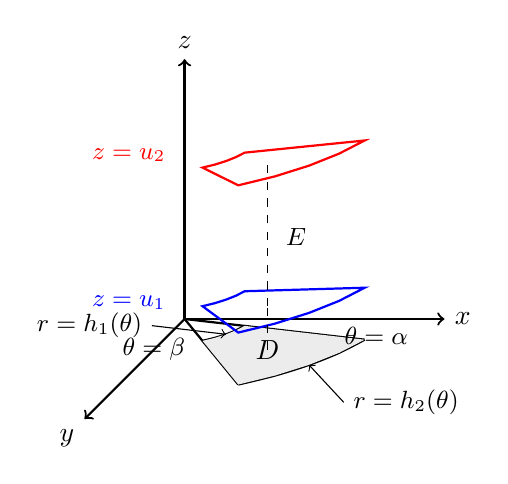
\begin{tikzpicture}[scale=1.1]
    \draw[thick,->] (0,0,0) -- (3,0,0) node[right]{$x$};
    \draw[thick,->] (0,0,0) -- (0,3,0) node[above]{$z$};
    \draw[thick,->] (0,0,0) -- (0,0,3) node[below left]{$y$};
    % wedge projection D in the y=0 plane (ground)
    % radial edges from origin
    \draw[thick] (0,0,0) -- ({2.4*cos(15)},0,{2.4*sin(15)});
    \draw[thick] (0,0,0) -- ({2.4*cos(55)},0,{2.4*sin(55)});
    % inner arc r=h1 (sampled points in 3D)
    \draw[thick] plot[smooth] coordinates {
        ({0.8*cos(15)},0,{0.8*sin(15)})
        ({0.8*cos(25)},0,{0.8*sin(25)})
        ({0.8*cos(35)},0,{0.8*sin(35)})
        ({0.8*cos(45)},0,{0.8*sin(45)})
        ({0.8*cos(55)},0,{0.8*sin(55)})
    };
    % outer arc r=h2
    \draw[thick] plot[smooth] coordinates {
        ({2.4*cos(15)},0,{2.4*sin(15)})
        ({2.4*cos(25)},0,{2.4*sin(25)})
        ({2.4*cos(35)},0,{2.4*sin(35)})
        ({2.4*cos(45)},0,{2.4*sin(45)})
        ({2.4*cos(55)},0,{2.4*sin(55)})
    };
    % fill the wedge region
    \fill[gray!15]
        ({0.8*cos(15)},0,{0.8*sin(15)})
        \foreach \a in {25,35,45,55} { -- ({0.8*cos(\a)},0,{0.8*sin(\a)}) }
        -- ({2.4*cos(55)},0,{2.4*sin(55)})
        \foreach \a in {45,35,25,15} { -- ({2.4*cos(\a)},0,{2.4*sin(\a)}) }
        -- cycle;
    \node at ({1.6*cos(35)},0,{1.6*sin(35)}) {$D$};
    % angle labels
    \node[below] at ({1.2*cos(5)+1},0,{1.2*sin(5)-0.15}) {\small$\theta=\alpha$};
    \node[left] at ({1.0*cos(55)-0.1},0,{1.0*sin(55)+0.1}) {\small$\theta=\beta$};
    % arc labels
    \draw[<-] ({0.8*cos(35)},0,{0.8*sin(35)}) -- (-0.3,0,0.2)
        node[left]{\small$r=h_1(\theta)$};
    \draw[<-] ({2.4*cos(35)},0,{2.4*sin(35)}) -- (2.8,0,2.5)
        node[right]{\small$r=h_2(\theta)$};
    % lower surface over wedge
    \draw[thick,blue]
        ({0.8*cos(15)},0.4,{0.8*sin(15)})
        \foreach \a in {25,35,45,55} { -- ({0.8*cos(\a)},0.4,{0.8*sin(\a)}) }
        -- ({2.4*cos(55)},0.6,{2.4*sin(55)})
        \foreach \a in {45,35,25,15} { -- ({2.4*cos(\a)},0.6,{2.4*sin(\a)}) }
        -- cycle;
    \node[blue,left] at (0.2,0.5,0.8) {\small$z=u_1$};
    % upper surface over wedge
    \draw[thick,red]
        ({0.8*cos(15)},2.0,{0.8*sin(15)})
        \foreach \a in {25,35,45,55} { -- ({0.8*cos(\a)},2.0,{0.8*sin(\a)}) }
        -- ({2.4*cos(55)},2.3,{2.4*sin(55)})
        \foreach \a in {45,35,25,15} { -- ({2.4*cos(\a)},2.3,{2.4*sin(\a)}) }
        -- cycle;
    \node[red,left] at (0.2,2.2,0.8) {\small$z=u_2$};
    % vertical dashed line at sample point
    \draw[dashed] ({1.6*cos(35)},0,{1.6*sin(35)})
        -- ({1.6*cos(35)},0.5,{1.6*sin(35)});
    \draw[dashed] ({1.6*cos(35)},0.5,{1.6*sin(35)})
        -- ({1.6*cos(35)},2.15,{1.6*sin(35)});
    \node[right] at ({1.6*cos(35)+0.1},1.3,{1.6*sin(35)}) {\small$E$};
\end{tikzpicture}
\end{center}

\[
    \iiint_E f\dd{V}
    = \iint_D\!\left(\int_{u_1}^{u_2} f\dd{z}\right)dA
\]
where $dA = \dd{x} \dd{y} = r\dd{r}\dd{\theta}$

\subsubsection{Spherical Coordinates}

\begin{definition}{Spherical Coordinates}{spherical-coord}
Spherical coordinates $(\rho, \theta, \varphi)$ (radius, longitude, latitude). Conversion formulas ($r = \sqrt{x^2+y^2} = \rho\sin\varphi$ is the distance to the $z$-axis):
\begin{align*}
    x &= r\cos\theta = \rho\sin\varphi\cos\theta \\
    y &= r\sin\theta = \rho\sin\varphi\sin\theta \\
    z &= \rho\cos\varphi
\end{align*}
\end{definition}

\begin{center}
	\begin{tikzpicture}[scale=1]
		\begin{axis}[
			view={100}{30},
			axis lines=center,
			width=12cm, height=10cm,
			xmin=0, xmax=5, ymin=0, ymax=6, zmin=0, zmax=5,
			xtick=\empty, ytick=\empty, ztick=\empty,
			xlabel={$x$}, ylabel={$y$}, zlabel={$z$},
			every axis x label/.style={at={(ticklabel* cs:1)},anchor=north east},
			every axis y label/.style={at={(ticklabel* cs:1)},anchor=north west},
			every axis z label/.style={at={(ticklabel* cs:1)},anchor=south},
			clip=false,
			trig format plots=deg
			]
			
			% Define coordinates
			\coordinate (O) at (0,0,0);
			\coordinate (P) at (3,4,4);
			\coordinate (Pxy) at (3,4,0);
			\coordinate (Pz) at (0,0,4);
			
			% Draw dashed projection lines
			\draw[dashed] (P) -- (Pxy);
			\draw[dashed] (Pz) -- (P) node[midway, above right] {$r = \sqrt{x^2+y^2} = \rho \sin\phi$};
			
			% Draw main vectors
			\draw[thick, ->] (O) -- (P) node[midway, above left] {$\rho$};
			\draw[thick, ->] (O) -- (Pxy);
			
			% Draw Point P
			\filldraw (P) circle (1.5pt) node[right] {$P$};
			
			% Draw theta arc (in xy plane, from x-axis to r)
			\addplot3 [
			forget plot,
			no marks,
			samples y=0,
			domain=0:53.13,
			samples=30,
			->
			] ({2*cos(x)}, {2*sin(x)}, 0);
			\node at ({2.6*cos(26.5)}, {2.6*sin(26.5)}, 0) {$\theta$};
			
			% Draw phi arc (from z-axis to rho vector)
			\addplot3 [
			forget plot,
			no marks,
			samples y=0,
			domain=0:51.3,
			samples=30,
			->
			] ({2.5*sin(x)*0.6}, {2.5*sin(x)*0.8}, {2.5*cos(x)});
			\node at ({3.1*sin(25)*0.6}, {3.1*sin(25)*0.8}, {3.1*cos(25)}) {$\phi$};
			
		\end{axis}
	\end{tikzpicture}
\end{center}

\textbf{Integration.} The volume element in spherical coordinates:
\[
    \dd{V} = \rho^2 \sin\varphi\;\dd{\rho}\dd{\theta}\dd{\varphi}
\]

\begin{center}
% Side view
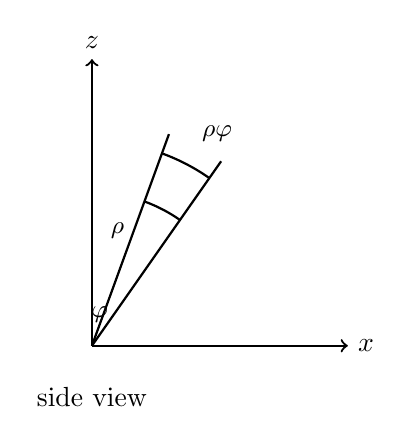
\begin{tikzpicture}[scale=1.3]
    \draw[thick,->] (0,0) -- (2.5,0) node[right]{$x$};
    \draw[thick,->] (0,0) -- (0,2.8) node[above]{$z$};
    % wedge
    \draw[thick] (0,0) -- ({2.2*cos(55)},{2.2*sin(55)});
    \draw[thick] (0,0) -- ({2.2*cos(70)},{2.2*sin(70)});
    % arcs at rho and rho+drho
    \draw[thick] ({1.5*cos(70)},{1.5*sin(70)}) arc[start angle=70, end angle=55, radius=1.5];
    \draw[thick] ({2.0*cos(70)},{2.0*sin(70)}) arc[start angle=70, end angle=55, radius=2.0];
    % labels
    \node[left] at ({1.2*cos(70)},{1.2*sin(70)}) {\small$\rho$};
    \node[right] at (-0.1, 0.3) {\small$\dd{\varphi}$};
    % dphi arc
    \node[right] at ({1.85*cos(58)},{1.85*sin(58)+0.5}) {\small$\rho\dd{\varphi}$};
    \node at (0,-0.5) {side view};
\end{tikzpicture}
\hspace{2cm}
% Top view
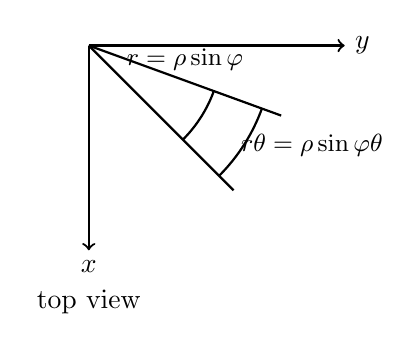
\begin{tikzpicture}[scale=1.3]
    \draw[thick,->] (0,0) -- (2.5,0) node[right]{$y$};
    \draw[thick,->] (0,0) -- (0,-2) node[below]{$x$};
    % wedge
    \draw[thick] (0,0) -- ({2.0*cos(20)},{-2.0*sin(20)});
    \draw[thick] (0,0) -- ({2.0*cos(45)},{-2.0*sin(45)});
    % arcs at r and r+dr
    \draw[thick] ({1.3*cos(45)},{-1.3*sin(45)}) arc[start angle=-45, end angle=-20, radius=1.3];
    \draw[thick] ({1.8*cos(45)},{-1.8*sin(45)}) arc[start angle=-45, end angle=-20, radius=1.8];
    % labels
    \node[above] at ({1.0*cos(20)},{-1.0*sin(20)}) {\small$r = \rho\sin\varphi$};
    \node[right] at ({1.7*cos(35)},{-1.7*sin(35)}) {\small$r\dd{\theta} = \rho\sin\varphi\dd{\theta}$};
    % dtheta label
    \node at (0,-2.5) {top view};
\end{tikzpicture}
\end{center}

\begin{example}
Describe the cone $z^2 = x^2 + y^2$ in both cylindrical and spherical coordinates.

\textbf{Cylindrical:} $r^2 = x^2 + y^2$, $z = z$, so the cone equation becomes $z^2 = r^2$.

\textbf{Spherical:} $r^2 = \rho^2\sin^2\varphi$, $z^2 = \rho^2\cos^2\varphi$, so
\[
    z^2 = r^2 \implies \sin^2\varphi = \cos^2\varphi
    \implies \tan^2\varphi = 1
    \implies \varphi = \frac{\pi}{4} \text{ or } \varphi = \frac{3\pi}{4}
\]
\end{example}

\begin{example}
Set up an integral to compute the volume of the solid enclosed by the cone $z = \sqrt{x^2+y^2}$ and the sphere $x^2+y^2+z^2 = 2$.

\begin{center}
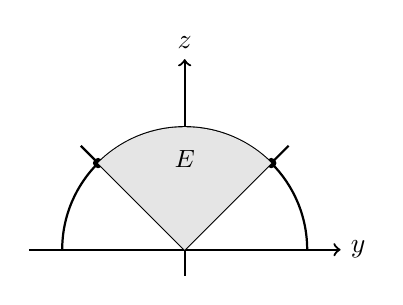
\begin{tikzpicture}[scale=1.1]
    \draw[thick,->] (-1.8,0) -- (1.8,0) node[right]{$y$};
    \draw[thick,->] (0,-0.3) -- (0,2.2) node[above]{$z$};
    % sphere arc
    \draw[thick] ({-sqrt(2)},0) arc[start angle=180, end angle=0, radius={sqrt(2)}];
    % cone
    \draw[thick] (0,0) -- (-1.2,1.2);
    \draw[thick] (0,0) -- (1.2,1.2);
    % intersection points
    \filldraw (1,1) circle (1.5pt);
    \filldraw (-1,1) circle (1.5pt);
    % shaded region
    \fill[gray!20] (0,0) -- (1,1) arc[start angle=45, end angle=135, radius={sqrt(2)}] -- cycle;
    \node at (0,1.05) {\small$E$};
\end{tikzpicture}
\end{center}

In cylindrical coordinates:
\begin{itemize}
    \item Cone: $z = r$
    \item Sphere: $r^2 + z^2 = 2 \implies z = \sqrt{2 - r^2}$
\end{itemize}
Intersection: $r^2 = 2 - r^2 \implies r = 1$, $z = 1$.

Shadow $D$: $r\in[0,1]$, $\theta\in[0,2\pi]$. \quad Vertical fiber: $z\in\bigl[r,\,\sqrt{2-r^2}\bigr]$.
\[
    \operatorname{Vol}(E)
    = \int_0^{2\pi}\!\int_0^1\!\int_r^{\sqrt{2-r^2}} r\dd{z}\dd{r}\dd{\theta}
\]

In spherical coordinates:
\begin{itemize}
    \item Cone: $\varphi = \dfrac{\pi}{4}$
    \item Sphere: $\rho = \sqrt{2}$
\end{itemize}
\[
    E = \left\{(\rho,\theta,\varphi) \;\middle|\; 0\leq\rho\leq\sqrt{2},\; 0\leq\theta\leq 2\pi,\; 0\leq\varphi\leq\frac{\pi}{4}\right\}
\]
\[
    \operatorname{Vol}(E)
    = \int_0^{\pi/4}\!\int_0^{2\pi}\!\int_0^{\sqrt{2}} \rho^2\sin\varphi\dd{\rho}\dd{\theta}\dd{\varphi}
\]
\end{example}

